\section{最小均方预测}
\label{sec:cexp-prediction}

到目前为止，条件期望只被描述为“保留累计期望的组内平均”。它还有一个优化的含义：如果只能根据已知信息去猜$X$，并以平方误差的平均衡量猜得好坏，最好的猜法就是条件期望。第~\ref{chap:random-vectors}章在形如$a+bx$的直线中找过最好的预测，这里不限定形式，允许使用已知信息的任意函数，只要求预测量平方可积。

设$X$平方可积。一个只用$\mathcal{G}$中信息的预测量是一个$\mathcal{G}$可测的随机变量$W$，要求$\mathbb{E}[W^{2}]<\infty$；它的\term{均方误差}（mean squared error）是$\mathbb{E}[(X-W)^{2}]$。问题是：在所有这样的$W$中，哪一个使均方误差最小？卷四的Hilbert空间投影给出了现成的框架。

\subsection{正交投影}
\label{sec:cexp-projection}

\paragraph{预测量组成的子空间}
平方可积随机变量组成$L^{2}=L^{2}(\Omega,\mathcal{F},\mathbb{P})$，内积为$\langle U,V\rangle=\mathbb{E}[UV]$，范数为$\lVert U\rVert_2=(\mathbb{E}[U^{2}])^{1/2}$。卷四证明了$L^{2}$是Hilbert空间，并且对Hilbert空间的闭线性子空间$M$与任一元素$f$，$M$中离$f$最近的元素存在且唯一，它由“$f$减去它与$M$正交”刻画，可参考\BookChapterRef{chap:function-inner-product-spaces}{卷四第12章“内积空间”}。

记
\[
 L^{2}(\mathcal{G})=\bigl\{W\in L^{2}:\ W\ \text{几乎必然等于某个}\ \mathcal{G}\ \text{可测的随机变量}\bigr\}.
\]
它是全体候选预测量。均方误差$\mathbb{E}[(X-W)^{2}]$就是$\lVert X-W\rVert_2^{2}$，所以最小均方预测是在$L^{2}(\mathcal{G})$中找离$X$最近的点。要用投影定理，先确认这个集合是闭线性子空间。

\begin{lemma}[已知信息上的平方可积变量]
\label{lem:cexp-closed-subspace}
$L^{2}(\mathcal{G})$是$L^{2}$的闭线性子空间。
\end{lemma}

\begin{proof}
$\mathcal{G}$可测的函数的线性组合仍$\mathcal{G}$可测，所以$L^{2}(\mathcal{G})$是线性子空间。

闭性借助完备性。$L^{2}(\mathcal{G})$中的元素与概率空间$(\Omega,\mathcal{G},\mathbb{P}_{\mathcal{G}})$上的平方可积函数一一对应，并且对$\mathcal{G}$可测的函数，对$\mathbb{P}_{\mathcal{G}}$与对$\mathbb{P}$的积分相同（见定理~\ref{thm:cexp-existence}的证明），所以这一对应保持范数。$L^{2}(\Omega,\mathcal{G},\mathbb{P}_{\mathcal{G}})$本身是Hilbert空间，因而完备。设$W_n\in L^{2}(\mathcal{G})$在$L^{2}$中收敛到$W$，则$(W_n)$是Cauchy列，在$L^{2}(\Omega,\mathcal{G},\mathbb{P}_{\mathcal{G}})$中收敛到某个$\mathcal{G}$可测的$W'$，也就在$L^{2}$中收敛到$W'$。极限唯一，$W=W'$几乎必然成立，所以$W\in L^{2}(\mathcal{G})$。
\end{proof}

这里不能简单地说“$\mathcal{G}$可测函数的极限仍$\mathcal{G}$可测”：$L^{2}$收敛只给出一个子列几乎必然收敛，而例外的零概率集未必属于$\mathcal{G}$。借助完备性绕开了这个问题。

\paragraph{残差与已知信息正交}
现在说明条件期望正是投影。思路是：把式~\eqref{eq:cexp-defining}中的示性函数$\mathbf{1}_{A}$换成一般的$W\in L^{2}(\mathcal{G})$。

\begin{theorem}[条件期望是正交投影]
\label{thm:cexp-projection}
设$X\in L^{2}$。则$\mathbb{E}[X\mid\mathcal{G}]\in L^{2}(\mathcal{G})$，并且对每个$W\in L^{2}(\mathcal{G})$，
\begin{equation}
 \mathbb{E}\bigl[(X-\mathbb{E}[X\mid\mathcal{G}])\,W\bigr]=0 .
 \label{eq:cexp-orthogonality}
\end{equation}
因此$\mathbb{E}[X\mid\mathcal{G}]$是$X$在$L^{2}(\mathcal{G})$上的正交投影。
\end{theorem}

\begin{proof}
记$Z=\mathbb{E}[X\mid\mathcal{G}]$。由定理~\ref{thm:cexp-lp}取$p=2$，$Z\in L^{2}$，它又是$\mathcal{G}$可测的，所以$Z\in L^{2}(\mathcal{G})$。

取$W\in L^{2}(\mathcal{G})$，不妨设$W$本身$\mathcal{G}$可测。由Cauchy--Schwarz不等式，
\[
 \mathbb{E}\lvert WX\rvert\leq\lVert W\rVert_2\lVert X\rVert_2<\infty ,
\]
所以$WX$可积。由提取已知量，$\mathbb{E}[WX\mid\mathcal{G}]=WZ$；两边取期望，由全期望公式，
\[
 \mathbb{E}[WX]=\mathbb{E}\bigl[\mathbb{E}[WX\mid\mathcal{G}]\bigr]=\mathbb{E}[WZ] .
\]
移项即得式~\eqref{eq:cexp-orthogonality}。$X-Z$与闭子空间$L^{2}(\mathcal{G})$正交，而$Z$在这个子空间中，由卷四的正交刻画，$Z$是$X$在其上的正交投影。
\end{proof}

正交条件~\eqref{eq:cexp-orthogonality}是积分刻画的推广。取$W=\mathbf{1}_{A}$，$A\in\mathcal{G}$，它就是式~\eqref{eq:cexp-defining}：残差$X-Z$在每个已知事件上的累计为零。反过来，若某个$Z\in L^{2}(\mathcal{G})$满足正交条件，取$W=\mathbf{1}_{A}$就知道它满足条件期望的定义。所以对平方可积的$X$，投影定理本身就给出了条件期望的存在性，不必经过Radon--Nikodym定理。这条路线只覆盖平方可积的情形；对只可积的$X$，存在性仍由定理~\ref{thm:cexp-existence}保证。

\paragraph{传感器表中的投影}
传感器表把这幅几何图景变成了有限维的计算。七个正概率格子上的函数组成一个七维空间，内积是按格子概率加权的乘积和。$\sigma(X)$可测的函数是在每行取常数的函数，组成一个三维子空间。$Y$在它上面的投影就是按行平均，残差$Y-\mathbb{E}[Y\mid X]$在每行内的加权和为零，因而与每一个行常数函数正交。

勾股定理给出平方长度的拆分。记$m(X)=\mathbb{E}[Y\mid X]$，第~\ref{chap:random-vectors}章已算得$\operatorname{Var}(Y)=0.6$、$\operatorname{Var}(m(X))=4/15$、平均条件方差为$1/3$，于是
\[
 \mathbb{E}[Y^{2}]=1.6,\qquad \mathbb{E}\bigl[m(X)^{2}\bigr]=\tfrac{4}{15}+1=\tfrac{19}{15},\qquad \mathbb{E}\bigl[(Y-m(X))^{2}\bigr]=\tfrac13 ,
\]
并且$\tfrac{19}{15}+\tfrac{5}{15}=\tfrac{24}{15}=1.6$。图~\ref{fig:cexp-projection}是这一关系的示意：$X$到平面$L^{2}(\mathcal{G})$的垂线足是$\mathbb{E}[X\mid\mathcal{G}]$。

\begin{BookInlineFigure}
  \centering
  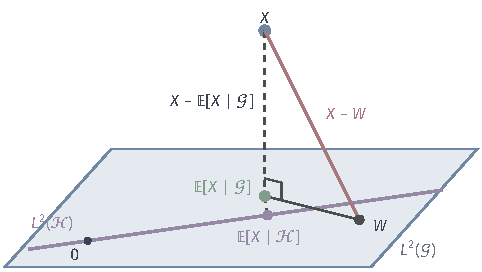
\includegraphics[width=82mm]{figures/07-probability/02-measure-theoretic-probability/tikz/cexp-projection/figure.pdf}
  \caption{条件期望是正交投影（示意）。浅蓝平面是$L^{2}(\mathcal{G})$，平面内的紫线是较小信息$\mathcal{H}\subseteq\mathcal{G}$对应的$L^{2}(\mathcal{H})$，常数（含$0$）都在其中。$X$的垂线足是$\mathbb{E}[X\mid\mathcal{G}]$（绿），残差（虚线）与平面垂直；平面中另一点$W$与$X$的距离（红）更长。再把$\mathbb{E}[X\mid\mathcal{G}]$投影到紫线上，得到$\mathbb{E}[X\mid\mathcal{H}]$。}
  \label{fig:cexp-projection}
\end{BookInlineFigure}

投影的观点也解释了塔式法则。$\mathcal{H}\subseteq\mathcal{G}$时$L^{2}(\mathcal{H})\subseteq L^{2}(\mathcal{G})$，先投影到大的子空间再投影到小的子空间，等于直接投影到小的子空间；先投影到小的子空间，结果已在大的子空间中，再投影到大的子空间不改变它。这正是式~\eqref{eq:cexp-tower}的两个等号在平方可积情形的几何含义。

\subsection{平方误差分解}
\label{sec:cexp-mse}

\paragraph{误差的勾股定理}
正交性直接给出任一预测量的误差构成。

\begin{theorem}[平方误差分解]
\label{thm:cexp-mse}
设$X\in L^{2}$，$Z=\mathbb{E}[X\mid\mathcal{G}]$。对每个$W\in L^{2}(\mathcal{G})$，
\begin{equation}
 \mathbb{E}\bigl[(X-W)^{2}\bigr]=\mathbb{E}\bigl[(X-Z)^{2}\bigr]+\mathbb{E}\bigl[(Z-W)^{2}\bigr].
 \label{eq:cexp-mse}
\end{equation}
因此$Z$在$L^{2}(\mathcal{G})$中使均方误差最小，并且使均方误差最小的$W$几乎必然等于$Z$。
\end{theorem}

\begin{proof}
把预测误差拆成两段：
\[
 X-W=(X-Z)+(Z-W).
\]
平方后取期望，交叉项是$2\,\mathbb{E}[(X-Z)(Z-W)]$。$Z-W\in L^{2}(\mathcal{G})$，由式~\eqref{eq:cexp-orthogonality}，交叉项为零，得到式~\eqref{eq:cexp-mse}。右边第二项非负，所以$\mathbb{E}[(X-W)^{2}]\geq\mathbb{E}[(X-Z)^{2}]$；等号成立当且仅当$\mathbb{E}[(Z-W)^{2}]=0$，即$W=Z$几乎必然成立。
\end{proof}

式~\eqref{eq:cexp-mse}把误差分成两部分：$\mathbb{E}[(X-Z)^{2}]$是已知信息无论如何也消除不了的部分，与$W$无关；$\mathbb{E}[(Z-W)^{2}]$是$W$偏离最佳预测而多付的代价。

用传感器表演示。取$\mathcal{G}=\sigma(X)$，再取一个较差的预测$W=\mathbb{E}[Y\mid\mathcal{H}]$，$\mathcal{H}=\sigma(\mathbf{1}_{\{X=2\}})$。它在前两行取$5/7$、第三行取$5/3$，是行常数函数，属于$L^{2}(\sigma(X))$。按行计算多付的代价：
\[
 \mathbb{E}\bigl[(Z-W)^{2}\bigr]=0.3\Bigl(\frac13-\frac57\Bigr)^{2}+0.4\Bigl(1-\frac57\Bigr)^{2}+0.3\cdot0=\frac{64}{1470}+\frac{16}{490}=\frac{8}{105}.
\]
再加上不可消除的部分$1/3$，
\[
 \mathbb{E}\bigl[(Y-W)^{2}\bigr]=\frac13+\frac{8}{105}=\frac{43}{105}\approx0.410 .
\]
直接按格子计算$(Y-W)^{2}$的加权和，也得到$43/105$。

\paragraph{信息多了，误差平均不增}
若$\mathcal{H}\subseteq\mathcal{G}$，则$\mathbb{E}[X\mid\mathcal{H}]\in L^{2}(\mathcal{H})\subseteq L^{2}(\mathcal{G})$，可以取它作为式~\eqref{eq:cexp-mse}中的$W$，得到
\begin{equation}
 \mathbb{E}\bigl[(X-\mathbb{E}[X\mid\mathcal{H}])^{2}\bigr]=\mathbb{E}\bigl[(X-\mathbb{E}[X\mid\mathcal{G}])^{2}\bigr]+\mathbb{E}\bigl[(\mathbb{E}[X\mid\mathcal{G}]-\mathbb{E}[X\mid\mathcal{H}])^{2}\bigr].
 \label{eq:cexp-information-monotone}
\end{equation}
更多的信息使最小均方误差不增，减少的量恰好是两个最佳预测之差的平方平均。上面的数值正是这一式的例子：只知道“是否偏高”时最小误差是$43/105$，知道完整的第一台读数后降到$1/3$。

这只是平均意义下的结论，不是逐个样本点的结论。图~\ref{fig:cexp-pointwise-error}比较七个正概率格子上的平方误差。格子$(0,1)$上$Y=1$，较粗的预测$5/7$误差为$4/49\approx0.08$，较细的预测$1/3$误差为$4/9\approx0.44$；格子$(1,0)$上误差也从约$0.51$增到$1$。信息变多后，这两个格子的预测变差了；但其他格子的改善更多，按概率加权后总体误差从$0.410$降到$0.333$。

\begin{BookInlineFigure}
  \centering
  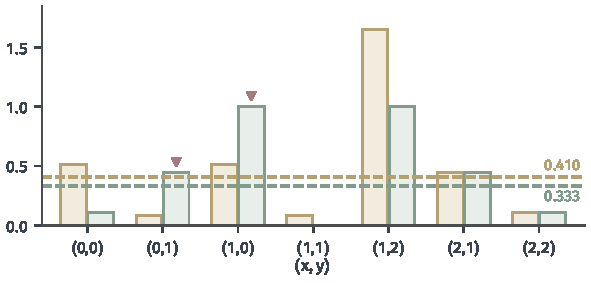
\includegraphics[width=100mm]{figures/07-probability/02-measure-theoretic-probability/matplotlib/cexp-pointwise-error/figure.pdf}
  \caption{逐格的平方误差，传感器表的七个正概率格子。黄柱：用$\mathbb{E}[Y\mid\mathcal{H}]$预测，$\mathcal{H}=\sigma(\mathbf{1}_{\{X=2\}})$；绿柱：用$\mathbb{E}[Y\mid X]$预测。红色三角标出信息增加后误差变大的格子$(0,1)$与$(1,0)$；两条虚线是按概率加权的平均误差$43/105\approx0.410$与$1/3$。}
  \label{fig:cexp-pointwise-error}
\end{BookInlineFigure}

最小化是在所有$\mathcal{G}$可测的平方可积预测量中进行的，不限于线性函数。传感器表与三角形模型中，$\mathbb{E}[Y\mid X]$恰好是$X$的线性函数，所以第~\ref{chap:random-vectors}章的最佳直线与这里的最佳预测重合。“只知绝对值”的例子中，$\mathrm{e}^{X}$的最佳预测$\cosh\lvert X\rvert$不是$\lvert X\rvert$的线性函数，最佳直线的均方误差就严格大于最佳预测的均方误差。从样本中估计这样的预测函数是统计推断的问题，可参考\BookChapterRef{chap:nonparametric-inference}{卷八第2章“非参数分布与函数推断”}。

\subsection{条件方差与全方差公式}
\label{sec:cexp-conditional-variance}

\paragraph{条件方差}
最小误差$\mathbb{E}[(X-Z)^{2}]$是一个数，它是对整个$\Omega$平均的结果。在每个已知群体内，残差平方的平均可以不同：传感器表中，第一行与第三行的条件方差是$2/9$，第二行是$1/2$。把残差平方再给定$\mathcal{G}$求条件期望，就得到随已知信息变化的波动大小。

\begin{definition}[条件方差]
\label{def:cexp-conditional-variance}
设$X\in L^{2}$，$Z=\mathbb{E}[X\mid\mathcal{G}]$。称
\begin{equation}
 \operatorname{Var}(X\mid\mathcal{G})=\mathbb{E}\bigl[(X-Z)^{2}\bigm|\mathcal{G}\bigr]
 \label{eq:cexp-conditional-variance}
\end{equation}
为$X$给定$\mathcal{G}$的条件方差。给定随机对象$Y$时取$\mathcal{G}=\sigma(Y)$，记作$\operatorname{Var}(X\mid Y)$。
\end{definition}

$(X-Z)^{2}$可积，因为$X,Z\in L^{2}$，所以定义有意义。它是$\mathcal{G}$可测的非负随机变量，只确定到零概率集。给定离散或有密度的$Y$时，第~\ref{chap:random-vectors}章的$v(y)=\operatorname{Var}(X\mid Y=y)$经过复合得到它的一个版本，理由与第~\ref{sec:cexp-given-variable}节的条件均值相同。

与不带条件的方差一样，条件方差有二阶矩的写法：
\begin{equation}
 \operatorname{Var}(X\mid\mathcal{G})=\mathbb{E}[X^{2}\mid\mathcal{G}]-\bigl(\mathbb{E}[X\mid\mathcal{G}]\bigr)^{2}.
 \label{eq:cexp-conditional-variance-moment}
\end{equation}
推导时把平方展开，$(X-Z)^{2}=X^{2}-2XZ+Z^{2}$，三项都可积，其中$XZ$的可积性由Cauchy--Schwarz不等式保证。对三项分别求条件期望，$Z$是已知量，由提取已知量，
\[
 \mathbb{E}[XZ\mid\mathcal{G}]=Z\,\mathbb{E}[X\mid\mathcal{G}]=Z^{2},\qquad \mathbb{E}[Z^{2}\mid\mathcal{G}]=Z^{2}.
\]
再由线性，
\[
 \operatorname{Var}(X\mid\mathcal{G})=\mathbb{E}[X^{2}\mid\mathcal{G}]-2Z^{2}+Z^{2}=\mathbb{E}[X^{2}\mid\mathcal{G}]-Z^{2}.
\]
由条件Jensen不等式，右边几乎必然非负，与定义一致。传感器表中，由第~\ref{sec:cexp-known}节的$\mathbb{E}[Y^{2}\mid X]$，第二行为$\tfrac32-1^{2}=\tfrac12$。

\needspace{8\baselineskip}
\paragraph{全方差公式}
有了条件方差，总方差可以拆成两部分。

\begin{theorem}[全方差公式]
\label{thm:cexp-total-variance}
设$X\in L^{2}$。则
\begin{equation}
 \operatorname{Var}(X)=\mathbb{E}\bigl[\operatorname{Var}(X\mid\mathcal{G})\bigr]+\operatorname{Var}\bigl(\mathbb{E}[X\mid\mathcal{G}]\bigr).
 \label{eq:cexp-total-variance}
\end{equation}
\end{theorem}

\begin{proof}
记$Z=\mathbb{E}[X\mid\mathcal{G}]$。常数$\mathbb{E}[X]$属于$L^{2}(\mathcal{G})$，在式~\eqref{eq:cexp-mse}中取$W=\mathbb{E}[X]$，
\[
 \mathbb{E}\bigl[(X-\mathbb{E}[X])^{2}\bigr]=\mathbb{E}\bigl[(X-Z)^{2}\bigr]+\mathbb{E}\bigl[(Z-\mathbb{E}[X])^{2}\bigr].
\]
左边是$\operatorname{Var}(X)$。右边第一项由全期望公式与式~\eqref{eq:cexp-conditional-variance}，
\[
 \mathbb{E}\bigl[(X-Z)^{2}\bigr]=\mathbb{E}\Bigl[\mathbb{E}\bigl[(X-Z)^{2}\bigm|\mathcal{G}\bigr]\Bigr]=\mathbb{E}\bigl[\operatorname{Var}(X\mid\mathcal{G})\bigr].
\]
由全期望公式$\mathbb{E}[Z]=\mathbb{E}[X]$，所以第二项是$\operatorname{Var}(Z)$。
\end{proof}

第一项是组内波动的平均，第二项是各组平均之间的波动。第~\ref{chap:random-vectors}章对概率表和联合密度分别证明过这个公式，现在它对任何信息都成立，证明只用到正交分解。

\paragraph{信息怎样重新分配方差}
总方差是固定的，信息只是在两项之间重新分配。图~\ref{fig:cexp-information-variance}(a)对传感器表的四层信息
\[
 \{\emptyset,\Omega\}\subseteq\mathcal{H}\subseteq\sigma(X)\subseteq\sigma(X,Y)
\]
画出这一分配。什么也不知道时，全部$0.6$都是组内波动；知道“是否偏高”时拆成$\tfrac{43}{105}+\tfrac{4}{21}$；知道第一台读数时拆成$\tfrac13+\tfrac{4}{15}$；知道两台读数时$Y$已知，全部是组间波动。由式~\eqref{eq:cexp-information-monotone}，组内波动的平均随信息增加而不增。$\mathcal{H}$这一层的组间部分可以直接算：$\mathbb{E}[Y\mid\mathcal{H}]$以概率$0.7,0.3$取$5/7,5/3$，均值为$1$，
\[
 \operatorname{Var}\bigl(\mathbb{E}[Y\mid\mathcal{H}]\bigr)=0.7\Bigl(\frac57-1\Bigr)^{2}+0.3\Bigl(\frac53-1\Bigr)^{2}=\frac{2}{35}+\frac{2}{15}=\frac{4}{21}.
\]

\begin{BookInlineFigure}
  \centering
  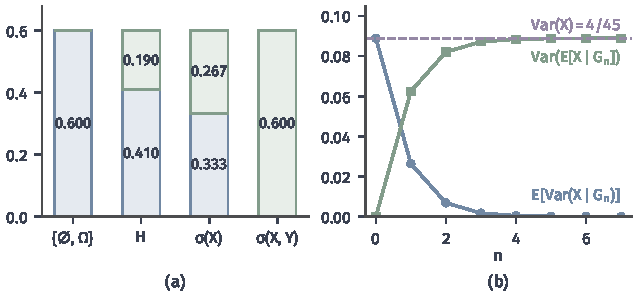
\includegraphics[width=108mm]{figures/07-probability/02-measure-theoretic-probability/matplotlib/cexp-information-variance/figure.pdf}
  \caption{全方差公式在信息增加时的分配。浅蓝或蓝色表示$\mathbb{E}[\operatorname{Var}(\cdot\mid\mathcal{G})]$，浅绿或绿色表示$\operatorname{Var}(\mathbb{E}[\cdot\mid\mathcal{G}])$。(a)传感器表中$Y$的方差$0.6$在四层信息下的拆分，$\mathcal{H}=\sigma(\mathbf{1}_{\{X=2\}})$。(b)$\Omega=[0,1)$，$X(\omega)=\omega^{2}$，$\mathcal{G}_n$为$2^{n}$等分，两部分之和恒为$\operatorname{Var}(X)=4/45$（紫色虚线）。}
  \label{fig:cexp-information-variance}
\end{BookInlineFigure}

逐次等分的例子给出一个连续的版本，见图~\ref{fig:cexp-information-variance}(b)。这里$X$的二阶矩是$\int_0^1\omega^{4}\,\mathrm{d}\omega=\tfrac15$，均值是$\tfrac13$，方差为$\tfrac15-\tfrac19=\tfrac4{45}$。$n=1$时，$\mathbb{E}[X\mid\mathcal{G}_1]$以各$\tfrac12$的概率取$\tfrac1{12}$与$\tfrac7{12}$，与均值$\tfrac13$各差$\tfrac14$，所以
\[
 \operatorname{Var}\bigl(\mathbb{E}[X\mid\mathcal{G}_1]\bigr)=\frac1{16},\qquad
 \mathbb{E}\bigl[\operatorname{Var}(X\mid\mathcal{G}_1)\bigr]=\frac4{45}-\frac1{16}=\frac{19}{720}\approx0.0264 .
\]
随着$n$增大，组间部分逐渐占据几乎全部方差，组内部分趋于零：分得越细，每段内$\omega^{2}$的变化越小。

\paragraph{平均下降，个别组可以上升}
与误差一样，“组内波动不增”只对平均成立。按读数之差$D$分组时，$\{D=0\}$组内$Y$等可能取$0,1,2$，
\[
 \operatorname{Var}(Y\mid D=0)=\frac{0+1+4}{3}-1^{2}=\frac23>0.6=\operatorname{Var}(Y).
\]
知道两台读数一致以后，第二台读数的波动反而比不加条件时更大；这一组的波动由另外两组较小的波动平衡，平均条件方差仍不超过$0.6$。
